\section{Experiment}
In this section, we conduct extensive experiments on different datasets which
contain the relatedness measured by human perceptions. We compute the Spearman
correlation coefficient between results of experiments and scores of human judgement
to evaluate the performance of our model. The model is implemented on 
Core-7-7700K@4.20GHz$\times$8 machine with 16GB memory and a archlinux platform.
 
\subsection{Dataset}
To evaluate models for semantic relatedness measurement, a common approach is to compare
the scores from the model and the scores provided by humans performing the same task.
This approach provides an model-independent way for evaluating measures of relatedness.
There are a good number of datasets which record the scores of human quantitative judgement
for semantic relatedness such as \emph{MC-30}\cite{MC30/Miller02}, \emph{RG-65}\cite{RG65/RubensteinG65}, 
\emph{REL-122}\cite{acl/SzumlanskiGS13}, \emph{MEN}\cite{MEN/BruniTB14}, 
\emph{YP-130}\cite{YP130/Yang06verbsimilarity}, \emph{WS}\cite{ws/AgirreAHKPS09},
\emph{wordsim-353}\cite{wordsim353/FinkelsteinGMRSWR02}
and so on. Some of these datasets are established with the measurement of 
similarity called \emph{similarity dataset}. Some others are \emph{relatedness dataset}.
Note that, all this datasets are English-language words.

1)\emph{similarity dataset}:
\emph{MC-30}, \emph{RG-65}, \emph{YP-130} and \emph{WS-353}are all established for computing similarity.
\emph{RG-65} is the classical similarity dataset which contains 65 pairs of words.
\emph{MC-30} contains 30 paris of words which is is the subset of \emph{RG-65}.
\emph{YP-130} is established for computing verb similarity which contains 130 pairs of verb.
\emph{wordsim353} contains two parts that are annotated by different groups of annotators.
The first set (set1) contains 153 word pairs along with their similarity scores assigned by 13 subjects. 
The second set (set2) contains 200 word pairs, with their similarity assessed by 16 subjects.
All these above are mere similarity datasets which just consider a particular case of relatedness.
There is another hybrid dataset \emph{WS} contains two sets of English word pairs along
with human-assigned similarity and relatedness judegements, called \emph{WS-sim} and \emph{WS-Rel} separately.
\emph{WS-sim} contains 203 paris of words along with similarity judgement,
and \emph{WS-rel} contains 252 along with relatedness judegement.

2)\emph{relatedness dataset}:
Compared to the similarity dataset, there are a small number of relatedness dataset such as
\emph{WS-Rel}, \emph{MEN} and \emph{REL-122}. \emph{WS-Rel} contains 252 pairs of words with
human-assigned relatedness judegements. \emph{MEN} contains 3000 paris of words which do not
instruct the subjects about the difference between similarity and relatedness. 
Dut the great number of human-assigned relatedness judegements, this collection can
be used to train and test computer algorithms implementing semantic similarity or relatedness measures.
We would not consider this collection in our experiments because of the illegibility of semantic measurement.
Another dataset \emph{REL-122} is a new relatedness norms which are a set of human-assigned relatedness scores
for 122 pairs of nouns.

The difference between similarity dataset and relatedness dataset is how human assigen the score for a
given pair of words. A common example is the pair of words \emph{"wheels-car"}. The \emph{wheels} is more related
with the \emph{car}, but they are dissimilar. \cite{acl/SzumlanskiGS13} created two additional experimental 
conditions in which subjects evaluated the Relatedness of noun pairs from the \emph{MC-30} study. We select 
ten pairs of words shown in table \ref{mc}. 

\begin{table}[]
    \centering
    \caption{Relatedness vs MC-30 similarity}
    \label{mc}
    \renewcommand\arraystretch{1.2}
    \setlength{\tabcolsep}{2.5mm}{
        \begin{tabular}{|lllll|}
        \hline
        \textbf{\#}  & \multicolumn{2}{l}{\textbf{Noun Pairs}} & \textbf{Sim.} & \textbf{Rel.} \\ \hline
        \textbf{1.}  & car              & automobile          & 3.92          & 4.00         \\
        \textbf{2.}  & gem              & jewel               & 3.84          & 3.98         \\
        \textbf{3.}  & coast            & shore               & 3.70          & 3.97         \\
        \textbf{4.}  & journey          & car                 & 1.16          & 3.00         \\
        \textbf{5.}  & forest           & graveyard           & 0.84          & 2.01         \\
        \textbf{6.}  & coast            & hill                & 0.87          & 1.59         \\
        \textbf{7.}  & shore            & woodland            & 0.63          & 1.63         \\
        \textbf{8.}  & lad              & wizard              & 0.42          & 2.12         \\
        \textbf{9.}  & crane            & implement           & 1.68          & 0.90         \\
        \textbf{10.} & noon             & string              & 0.08          & 0.14         \\ \hline
        \end{tabular}
    }
\end{table}
We can see that the relatedness for pairs that are related but
dissimilar(e.g., \emph{journey-car} and \emph{forest-graveyard}). 
This indicates that asking subjects to evaluate “similarity” instead of “relatedness” can
significantly impact the results in studies of semantic relatedness measurement.
However, previous researchs do not consider the semantic difference among some datasets.
For example, in \cite{ijcai/GabrilovichM07}, \cite{textgraphs/YehRMAS09}, \cite{aaai/Pirro12}
and so on, the researchers all regard the dataset \emph{MC-30} as relatedness dataset to conduct experiments.
Following these reasearch the similarity dataset \emph{MC-30} and \emph{RG-65} would be leveraged besides
the relatedness datasets such as \emph{rel-122} and \emph{WS-rel}. Moreover, we extract the relatedness
scores from \cite{acl/SzumlanskiGS13} which are shown in table \ref{mc} for dataset \emph{MC-30}.

For an given pair of words, we firstly get two sets of corresponding entities in DBPedia. 
Then we adopt a method of embedding to train the subgraph which is extracted from DBPedia
based on those entities. Finally,  we get multiple relatedness scores after
a join between two set of entities. In order to better fit the judgement of human, we utilize a
weighted strategy to combine multiple relatedness scores of pairwise entities.

\subsection{Parameter tuning}
We can recall from section \ref{sec:train} and \ref{sec:measure} that there are some parameter
which may have an impact on semantic relatedness measure. Such as, the final relatedness
socres would be affected by the dimension of vector of distributional representation
as well as the number of entities associated with given words.
Besides, we tune the $\alpha$ parameter for the \emph{weighted} strategy on \emph{WS-rel} dataset.
We pick \emph{WS-rel} since there are not many comparison systems in the literature that
report results on this dataset. Another reason is that the quantity of \emph{WS-rel} is more
greater than other datasets which is comprehensive for our parameter tuning.
Finally, we find the optimal values for $\alpha$ to be 7.

% For the impact for final score which is affected by the number of entities queried by given words, we
% show the variation trend of \emph{Spearman} correlation coefficient following the increase of queried entities.

As you can see by the line chart \ref{dim}, we exhibit the impact of dimension of learnt embedding
vector for relatedness measurement with \emph{closest} and \emph{weighted} strategy. 
We conduct this result based on datasets which consist of
\emph{MC-Rel-30}, \emph{MC-Sim-30}, \emph{RG-65}, \emph{rel-122}, and \emph{WS-rel}, and get the 
average values of the results in five datasets shown in the sixth line chart finally. It is obviously
that the we get the optimal relatedness scores when the dimension of vector is assigned to \emph{100}.

\begin{figure}
    \centering
    \subfigure[The impact of Dimension of vector for relatedness measure]{
        \label{dim}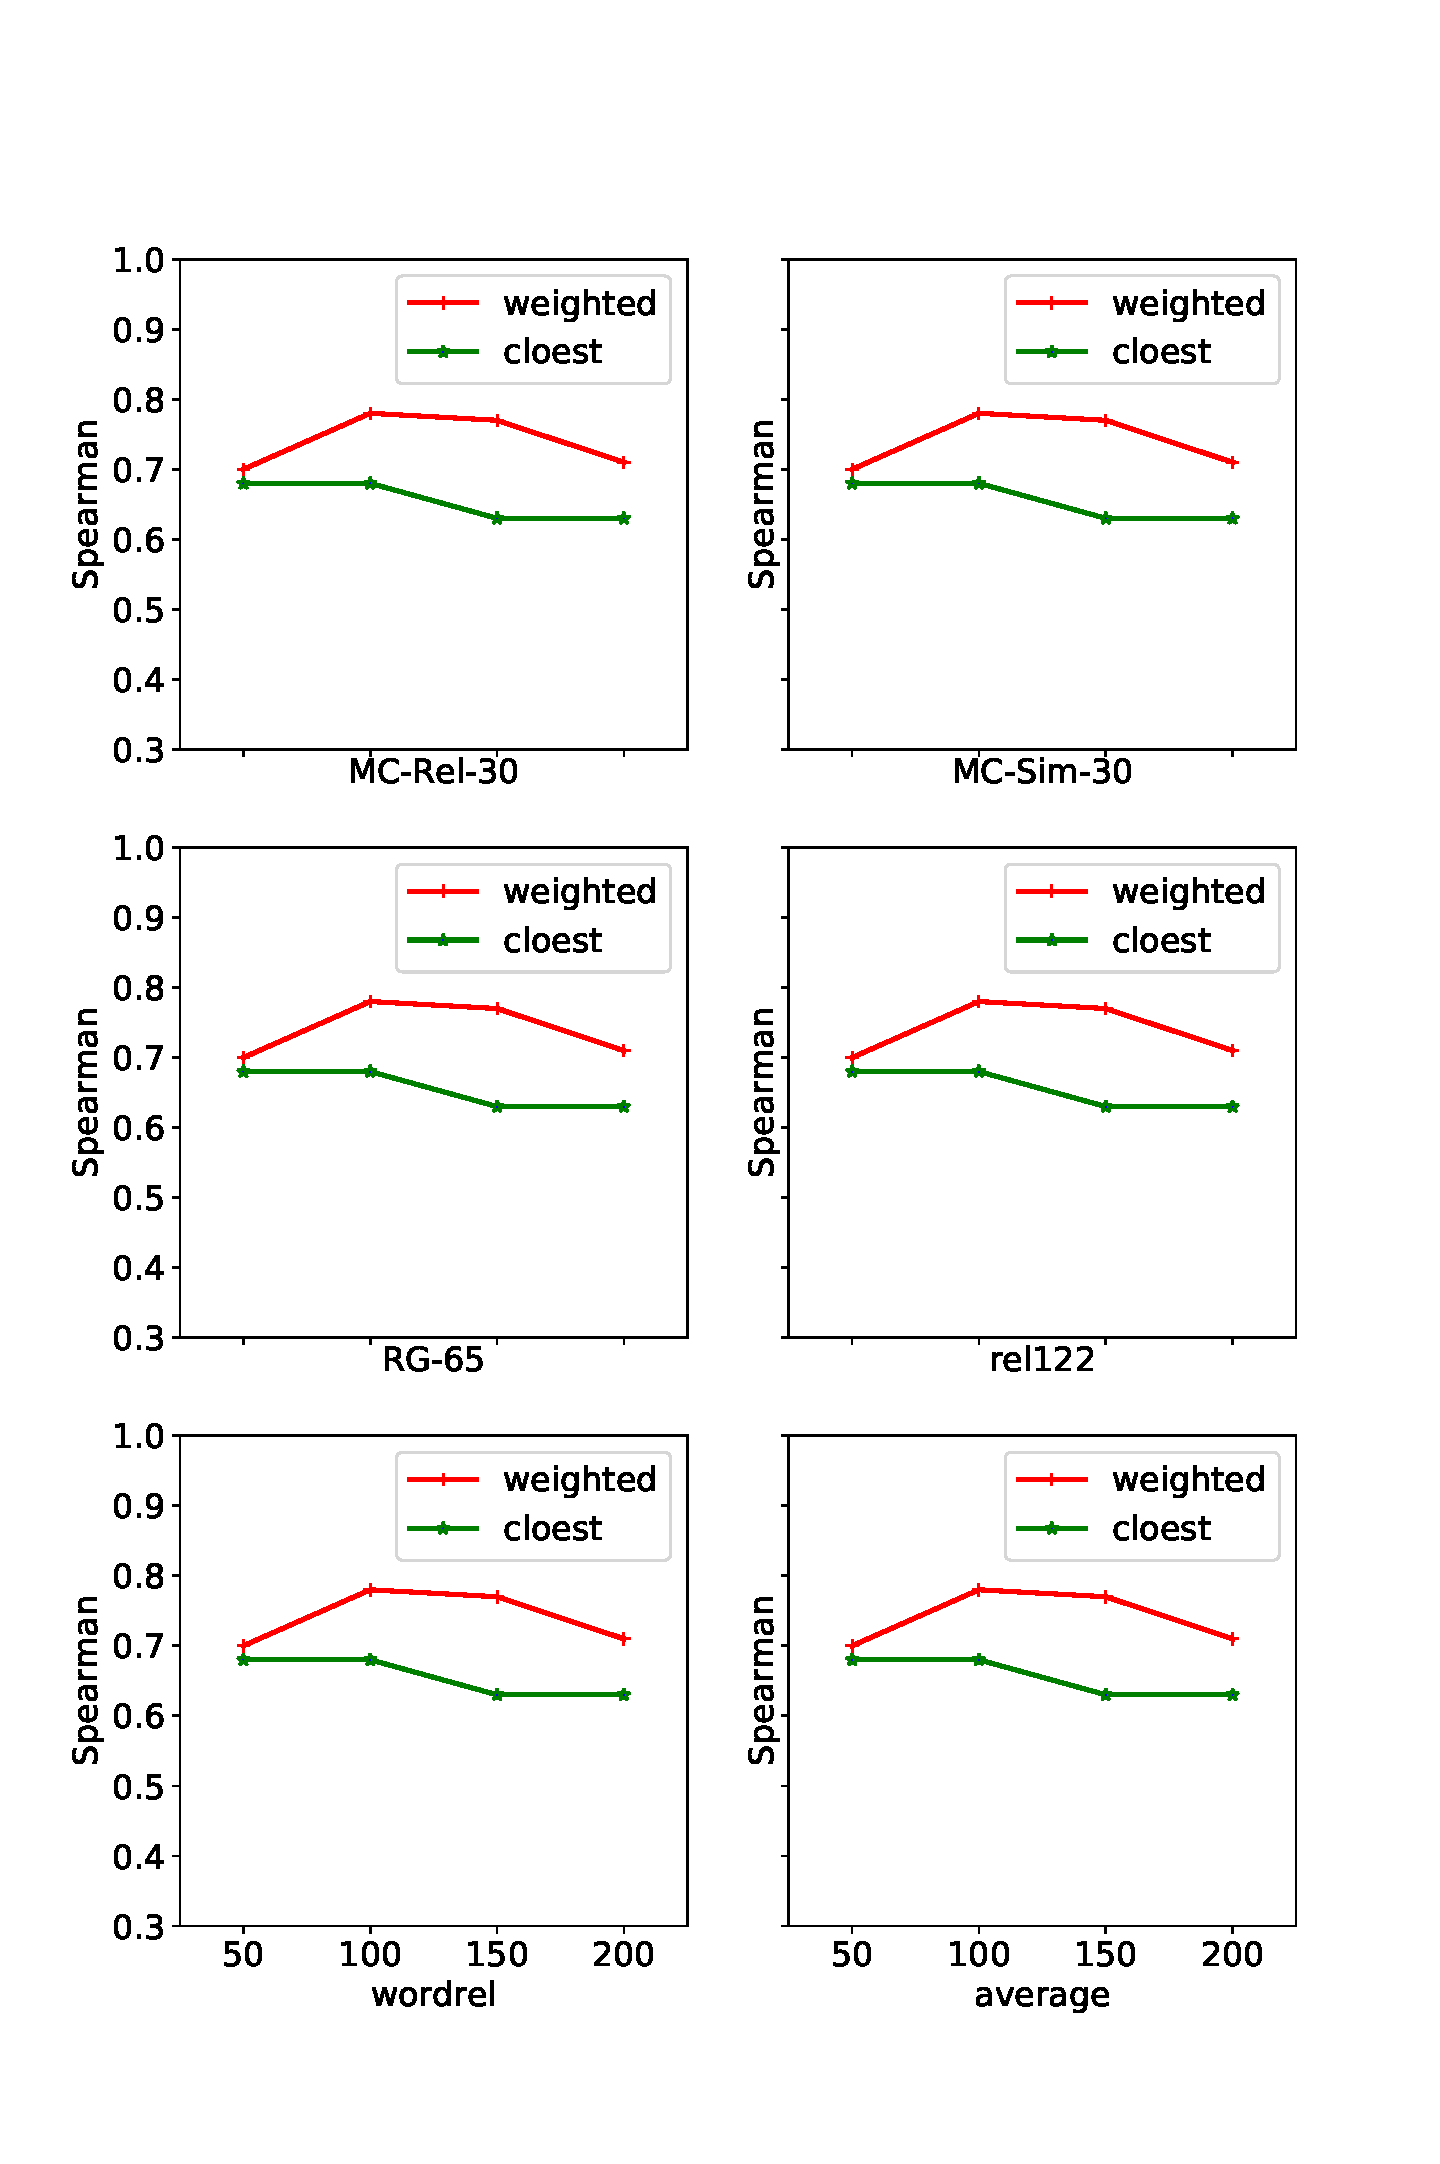
\includegraphics[width=55mm]{pic/dim.pdf}}
    \subfigure[The impact of the number of entities queried by given words]{
        \label{ent-num}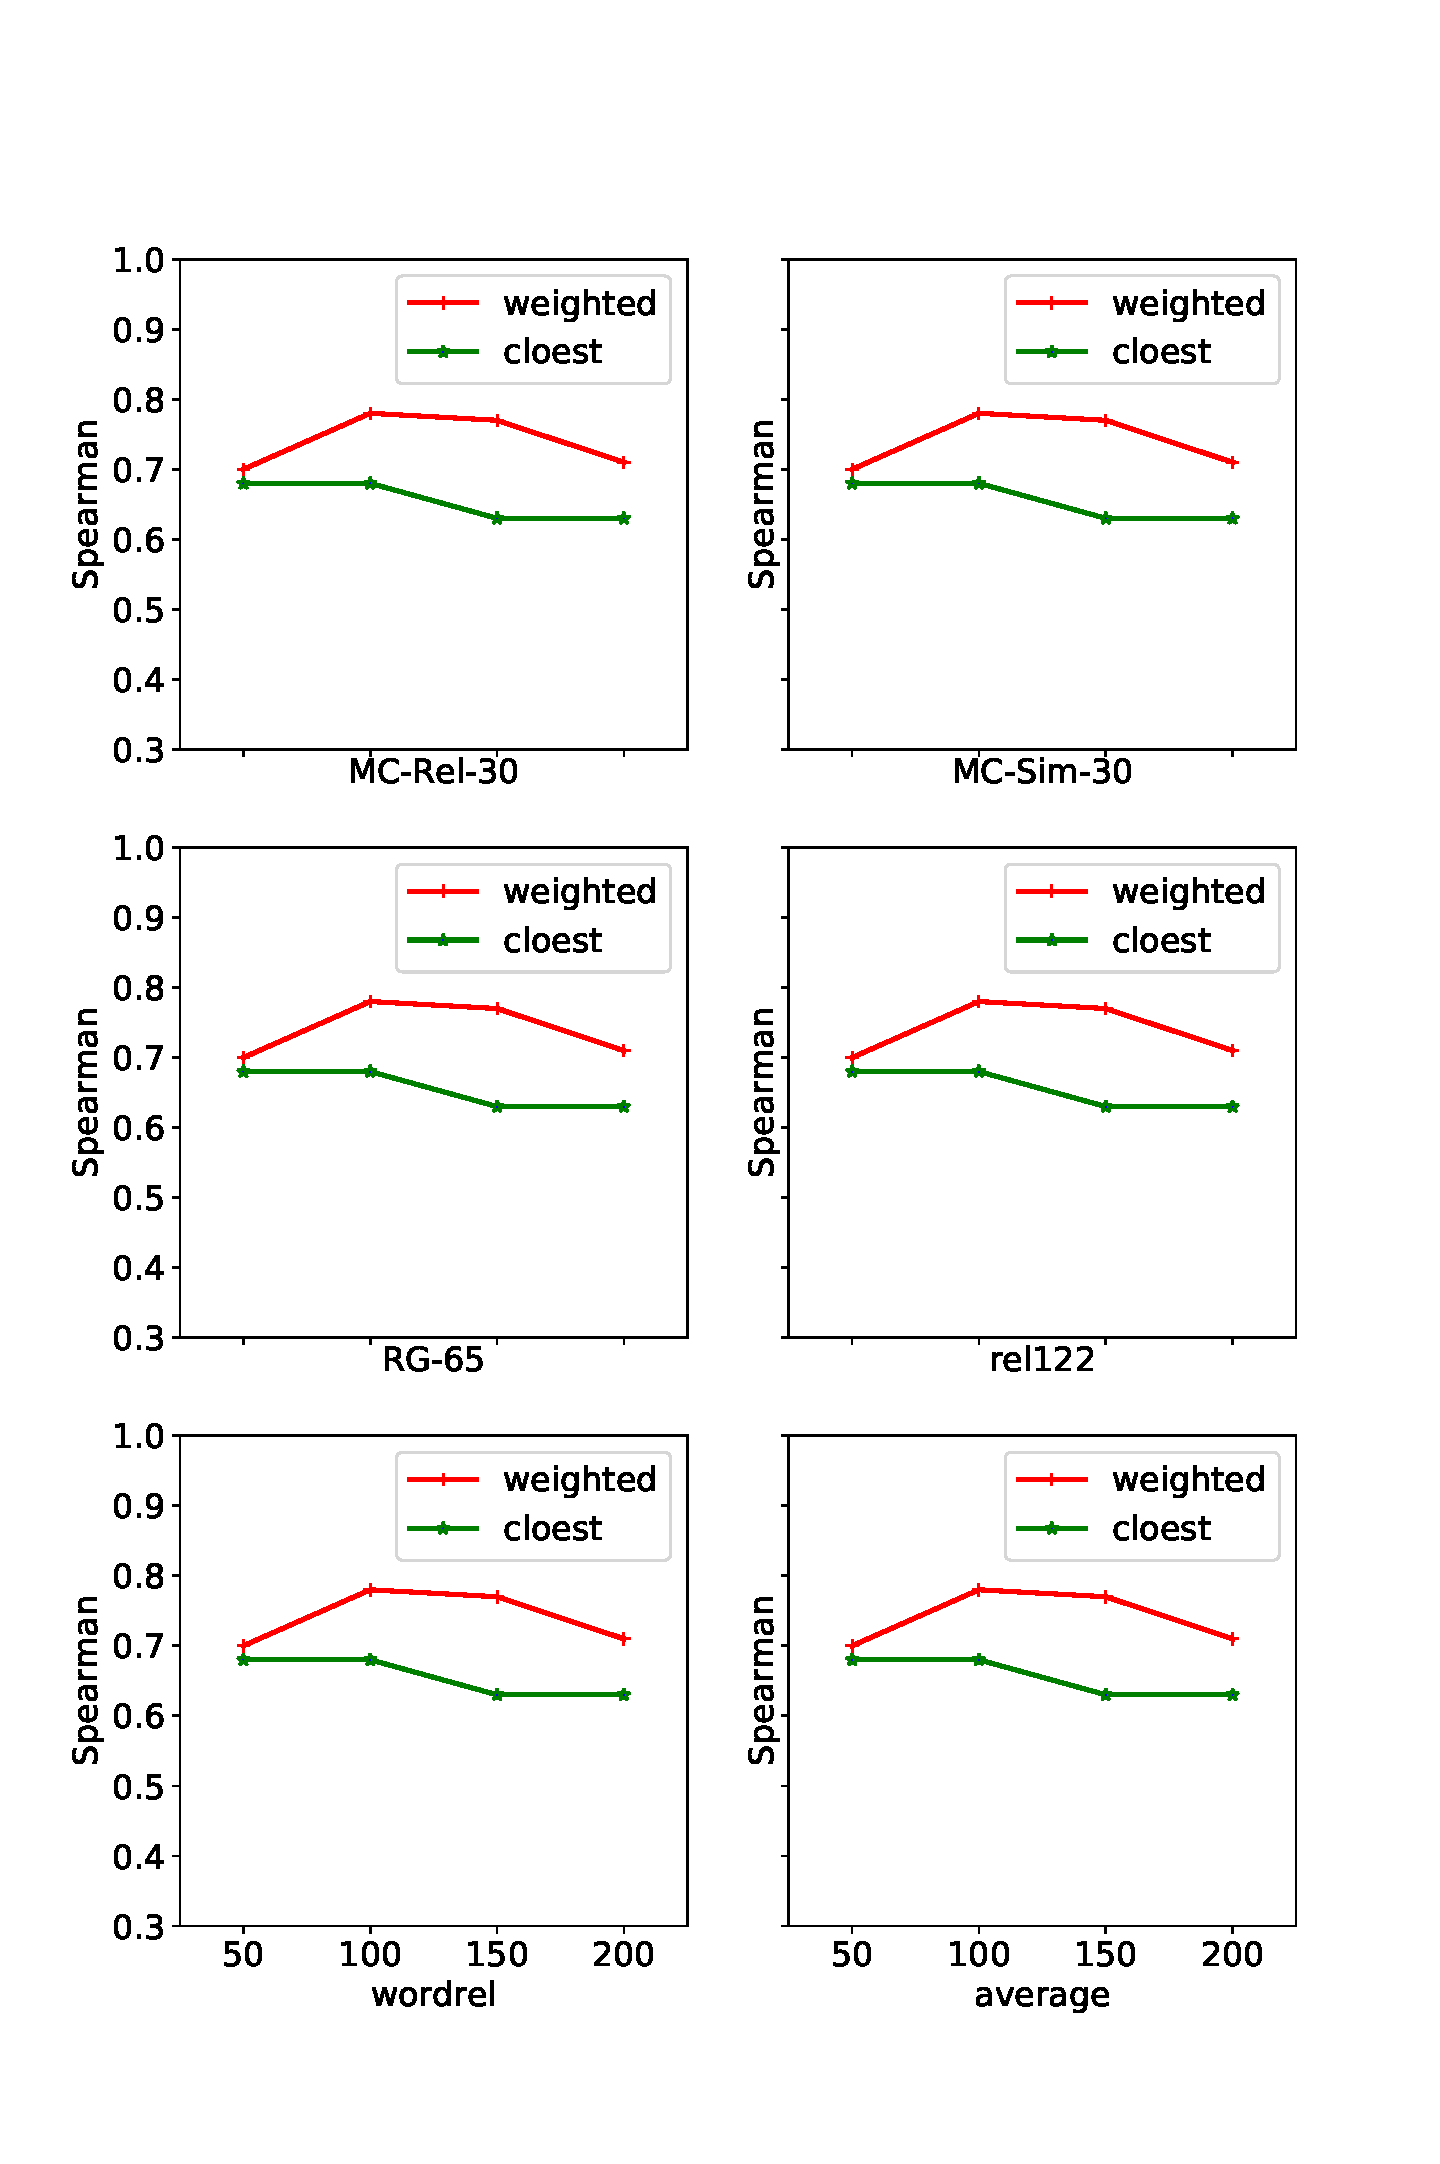
\includegraphics[width=55mm]{pic/dim.pdf}
    }
\end{figure}
%     \begin{minipage}[t][0.5\linewidth]
%         \centering
%         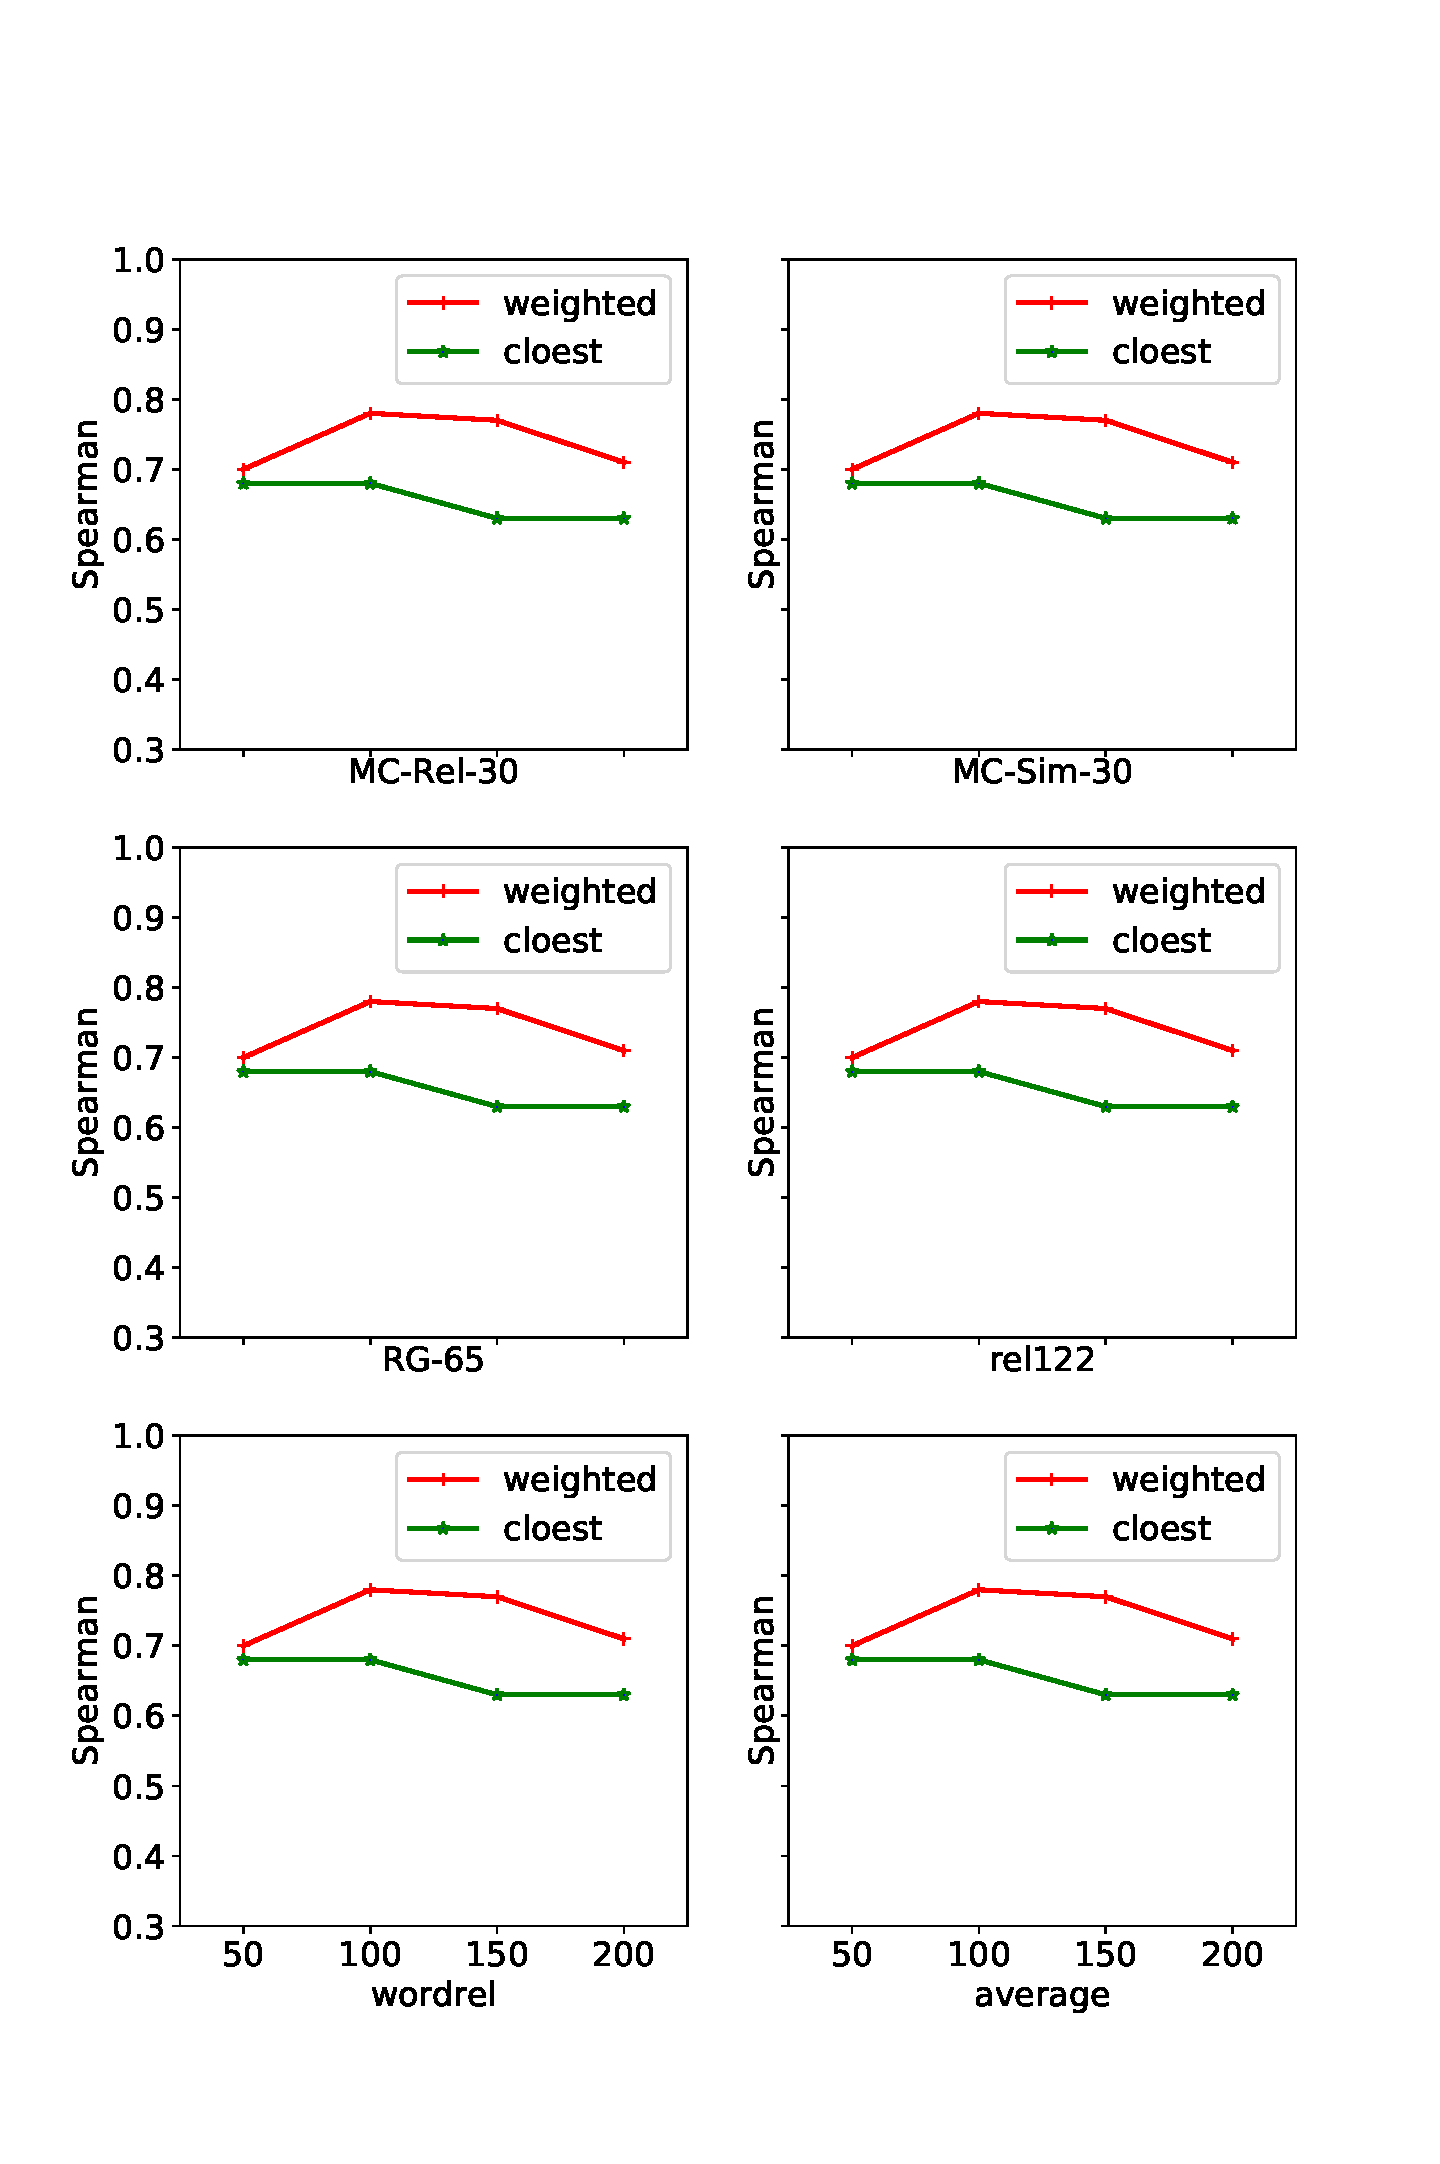
\includegraphics[width=0.53]{pic/dim.pdf}
%         \caption{The impact of Dimension of vector for relatedness measure}
%         \label{dim}
%     \end{minipage}

%     \begin{minipage}[t][0.5\linewidth]
%         \centering
%         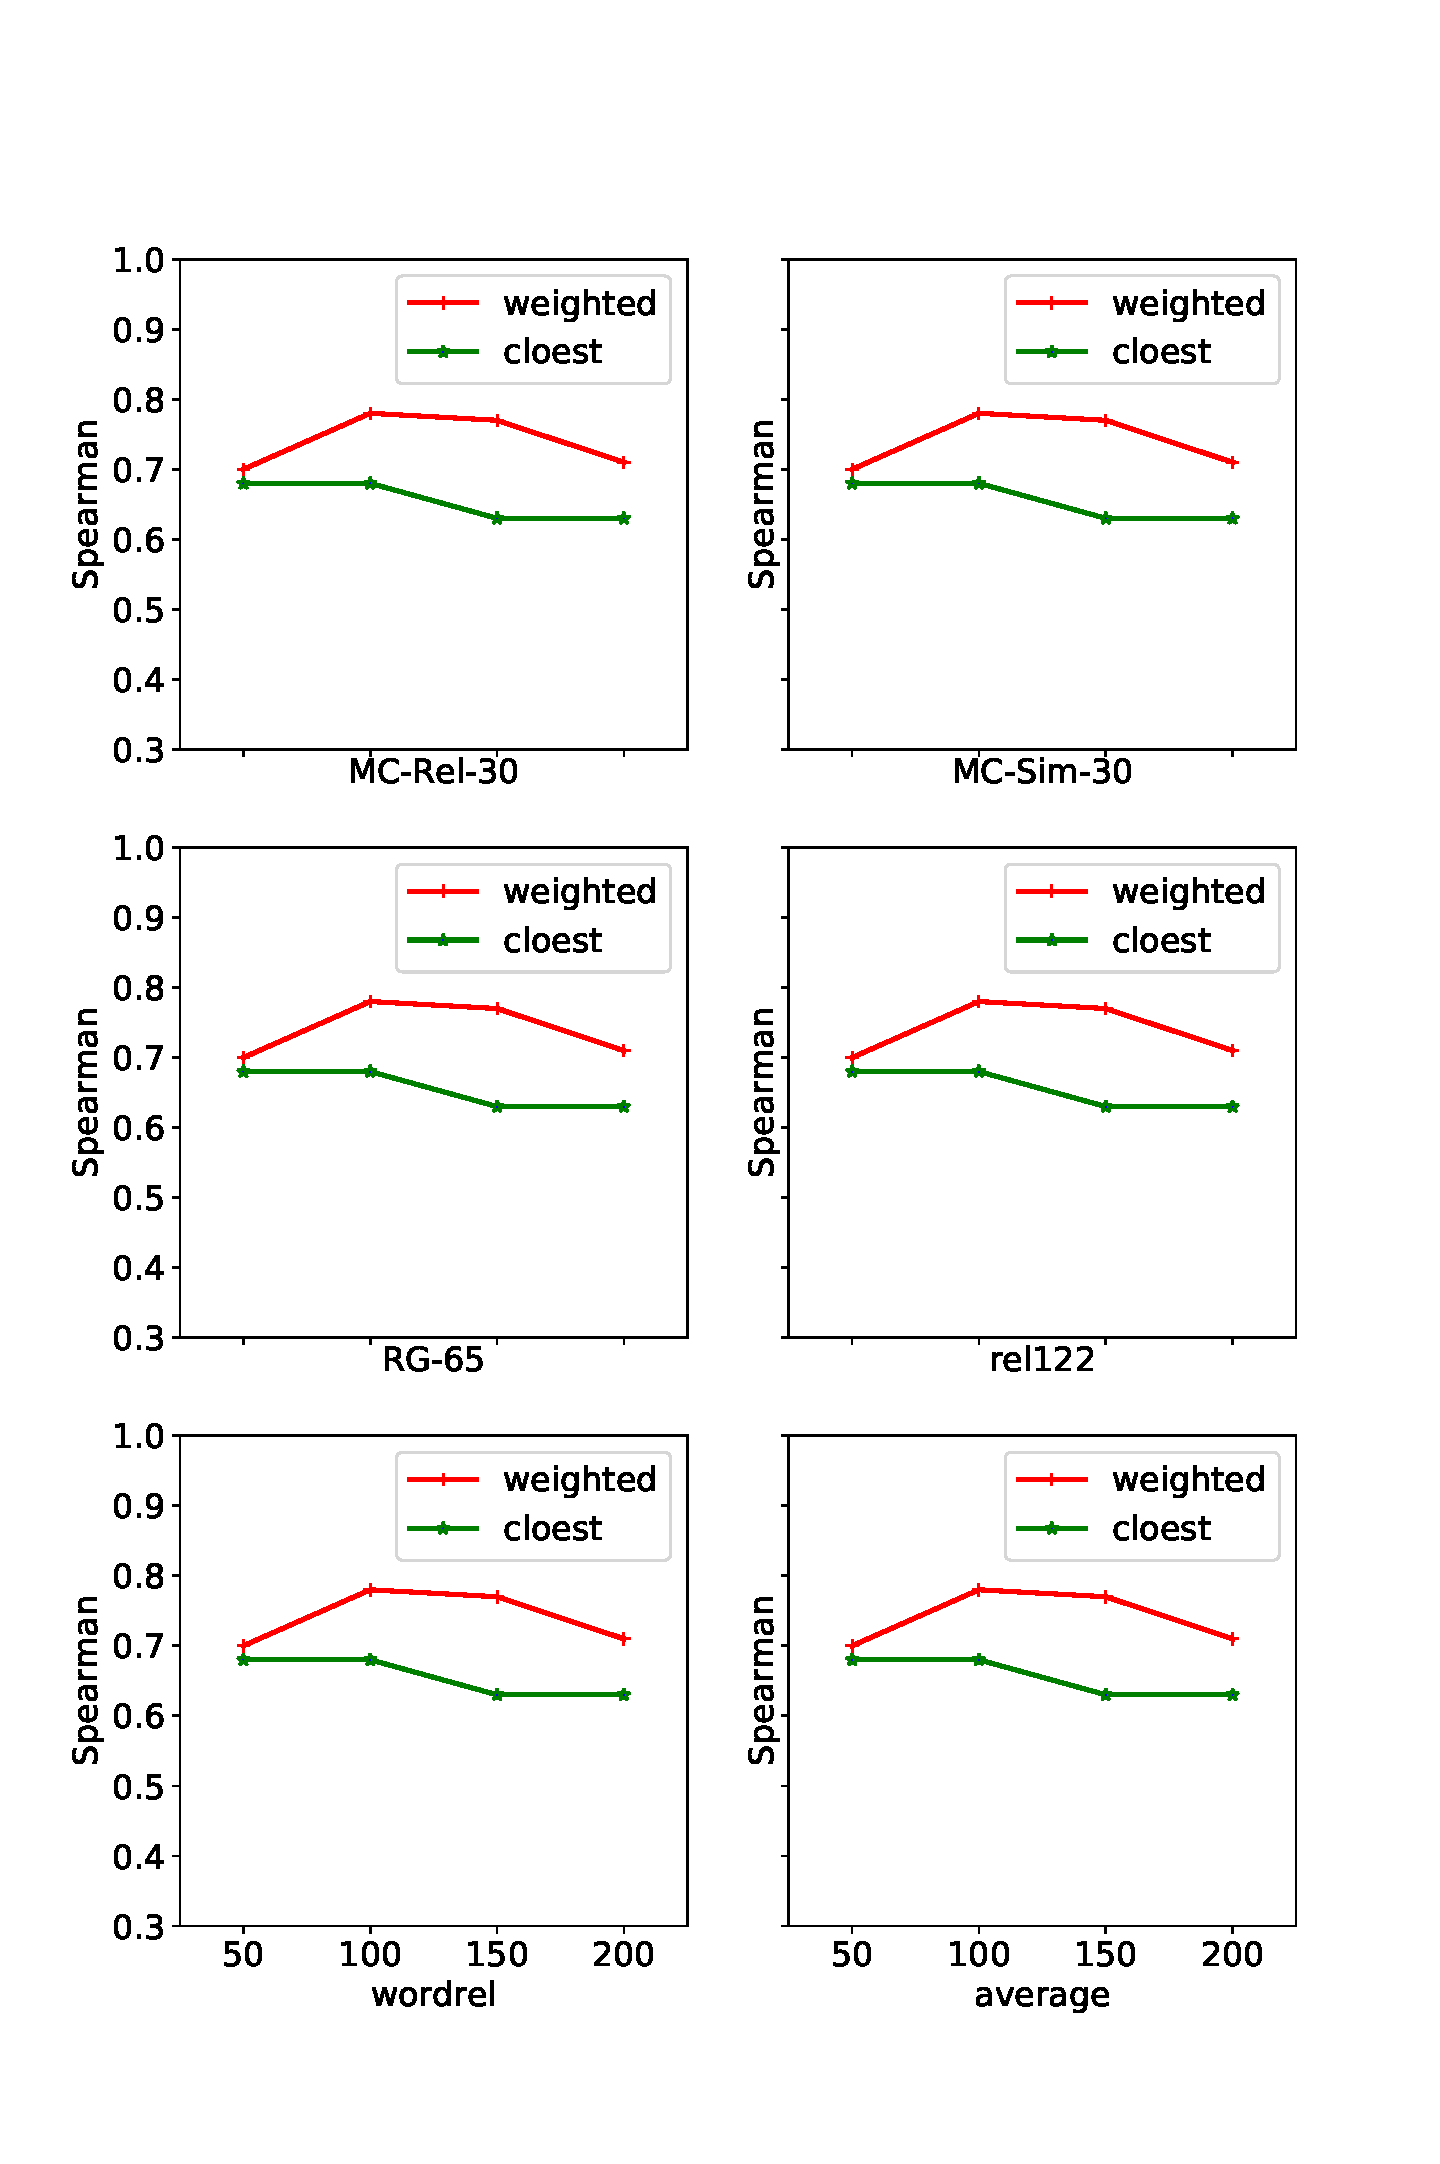
\includegraphics[width=0.53]{pic/dim.pdf}
%         \caption{The impact of the number of entities queried by given words}
%         \label{ent-num} 
%     \end{minipage}
% \end{figure}



In the figure \ref{ent-num}, following the dataset and measurement strategy, we draw the variation trend
of semantic relatedness scores following the increase of the quantity of entities queried by given words.
The slope of correlation coefficient curve rises gently with the increase of number of queried entities.
Distinguishingly, when the quantity of queried entities is greater than 5, the correlation coefficient
curve have a concave shown in pic \emph{X} because extra and overmuch entities would bring noise for the final
semantic relatedness socres

\begin{table}[H]
    \centering
    \caption{Spearman correlation performance on five word similarity and relatedness datasets}
    \label{spearman}
    \renewcommand\arraystretch{1.15}
    \setlength{\tabcolsep}{2.5mm}{
        \begin{tabular}{lcllccl}
        \hline
        \multirow{2}{*}{\textbf{Measure}} & \multicolumn{5}{c}{\textbf{Dataset}}                                                                                          & \textbf{} \\ \cline{2-6}
                                        & \multicolumn{1}{l}{MC-rel-30} & MC-30 & RG-65                  & \multicolumn{1}{l}{rel122} & \multicolumn{1}{l}{wordrel} & Averrage  \\ \hline
        \textbf{WikiRelate!}              & --                            & 0.45          & 0.52                   & --                         & --                          &           \\
        \textbf{ESA}                      & --                            & 0.75          & 0.82                   & --                         & --                          &           \\
        \textbf{WLM}                      & --                            & 0.70          & 0.64                   & --                         & --                          &           \\
        \textbf{WikiWalk}                 & --                            & 0.61          & \multicolumn{1}{c}{--} & --                         & --                          &           \\
        \textbf{REWOrD}                   & --                            & 0.72          & 0.78                   & --                         & --                          &           \\ \hline
        \textbf{Pando-closest}            & \multicolumn{1}{l}{}          & 0.81          &                        & \multicolumn{1}{l}{}       & \multicolumn{1}{l}{}        &           \\
        \textbf{Pando-weighted}           & \multicolumn{1}{l}{}          & \textbf{0.85} &                        & \multicolumn{1}{l}{}       & \multicolumn{1}{l}{}        &           \\ \hline
        \end{tabular}
    }
\end{table}

Compared to previous method of semantic relatedness measurement, we run our model on five dataset
\emph{MC-Rel-30}, \emph{MC-Sim-30}, \emph{RG-65}, \emph{rel-122}, and \emph{WS-rel}, and report the
\emph{Spearman} correlation coefficient performance for the two strategies of our model. It can been
seen that our model proves to be highly reliable on semantic relatedness measurement tasks, obtaining
the best performance on most datasets. In addition, our approach in dataset \emph{MC-Rel-30} out outperform
the results in dataset \emph{MC-Sim-30} which proves our model if more suitable for computing semantic
relatedness than similarity. 